\appendix
\addappheadtotoc
\counterwithin{figure}{section}
\section{Appendix}
\label{sec:sec010}

%%%%%%%%%%%%%%%%%%%%%%%%%%%%%%%%%%%%%%%%%%%%%%%%%%%
\begin{figure}[htbp]
\onecolumn
\centering
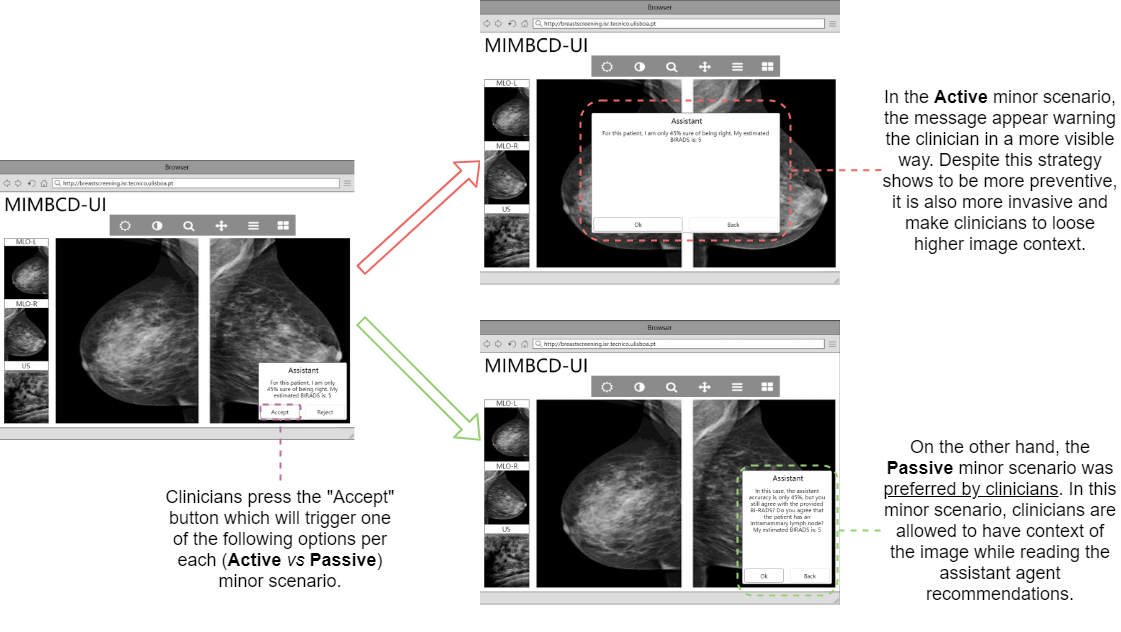
\includegraphics[width=0.95\textwidth]{fig022}
\caption{When the clinician press the "Accept" button, the system will trigger two minor scenario options: (a) {\bf Active}; or (b) {\bf Passive}. During our sessions of low-fi prototype co-design with clinicians, all of them preferred the (b) {\bf Passive} option.}
\label{fig:fig022}
\twocolumn
\end{figure}
%%%%%%%%%%%%%%%%%%%%%%%%%%%%%%%%%%%%%%%%%%%%%%%%%%%

%%%%%%%%%%%%%%%%%%%%%%%%%%%%%%%%%%%%%%%%%%%%%%%%%%%
\begin{figure}[htbp]
\onecolumn
\centering
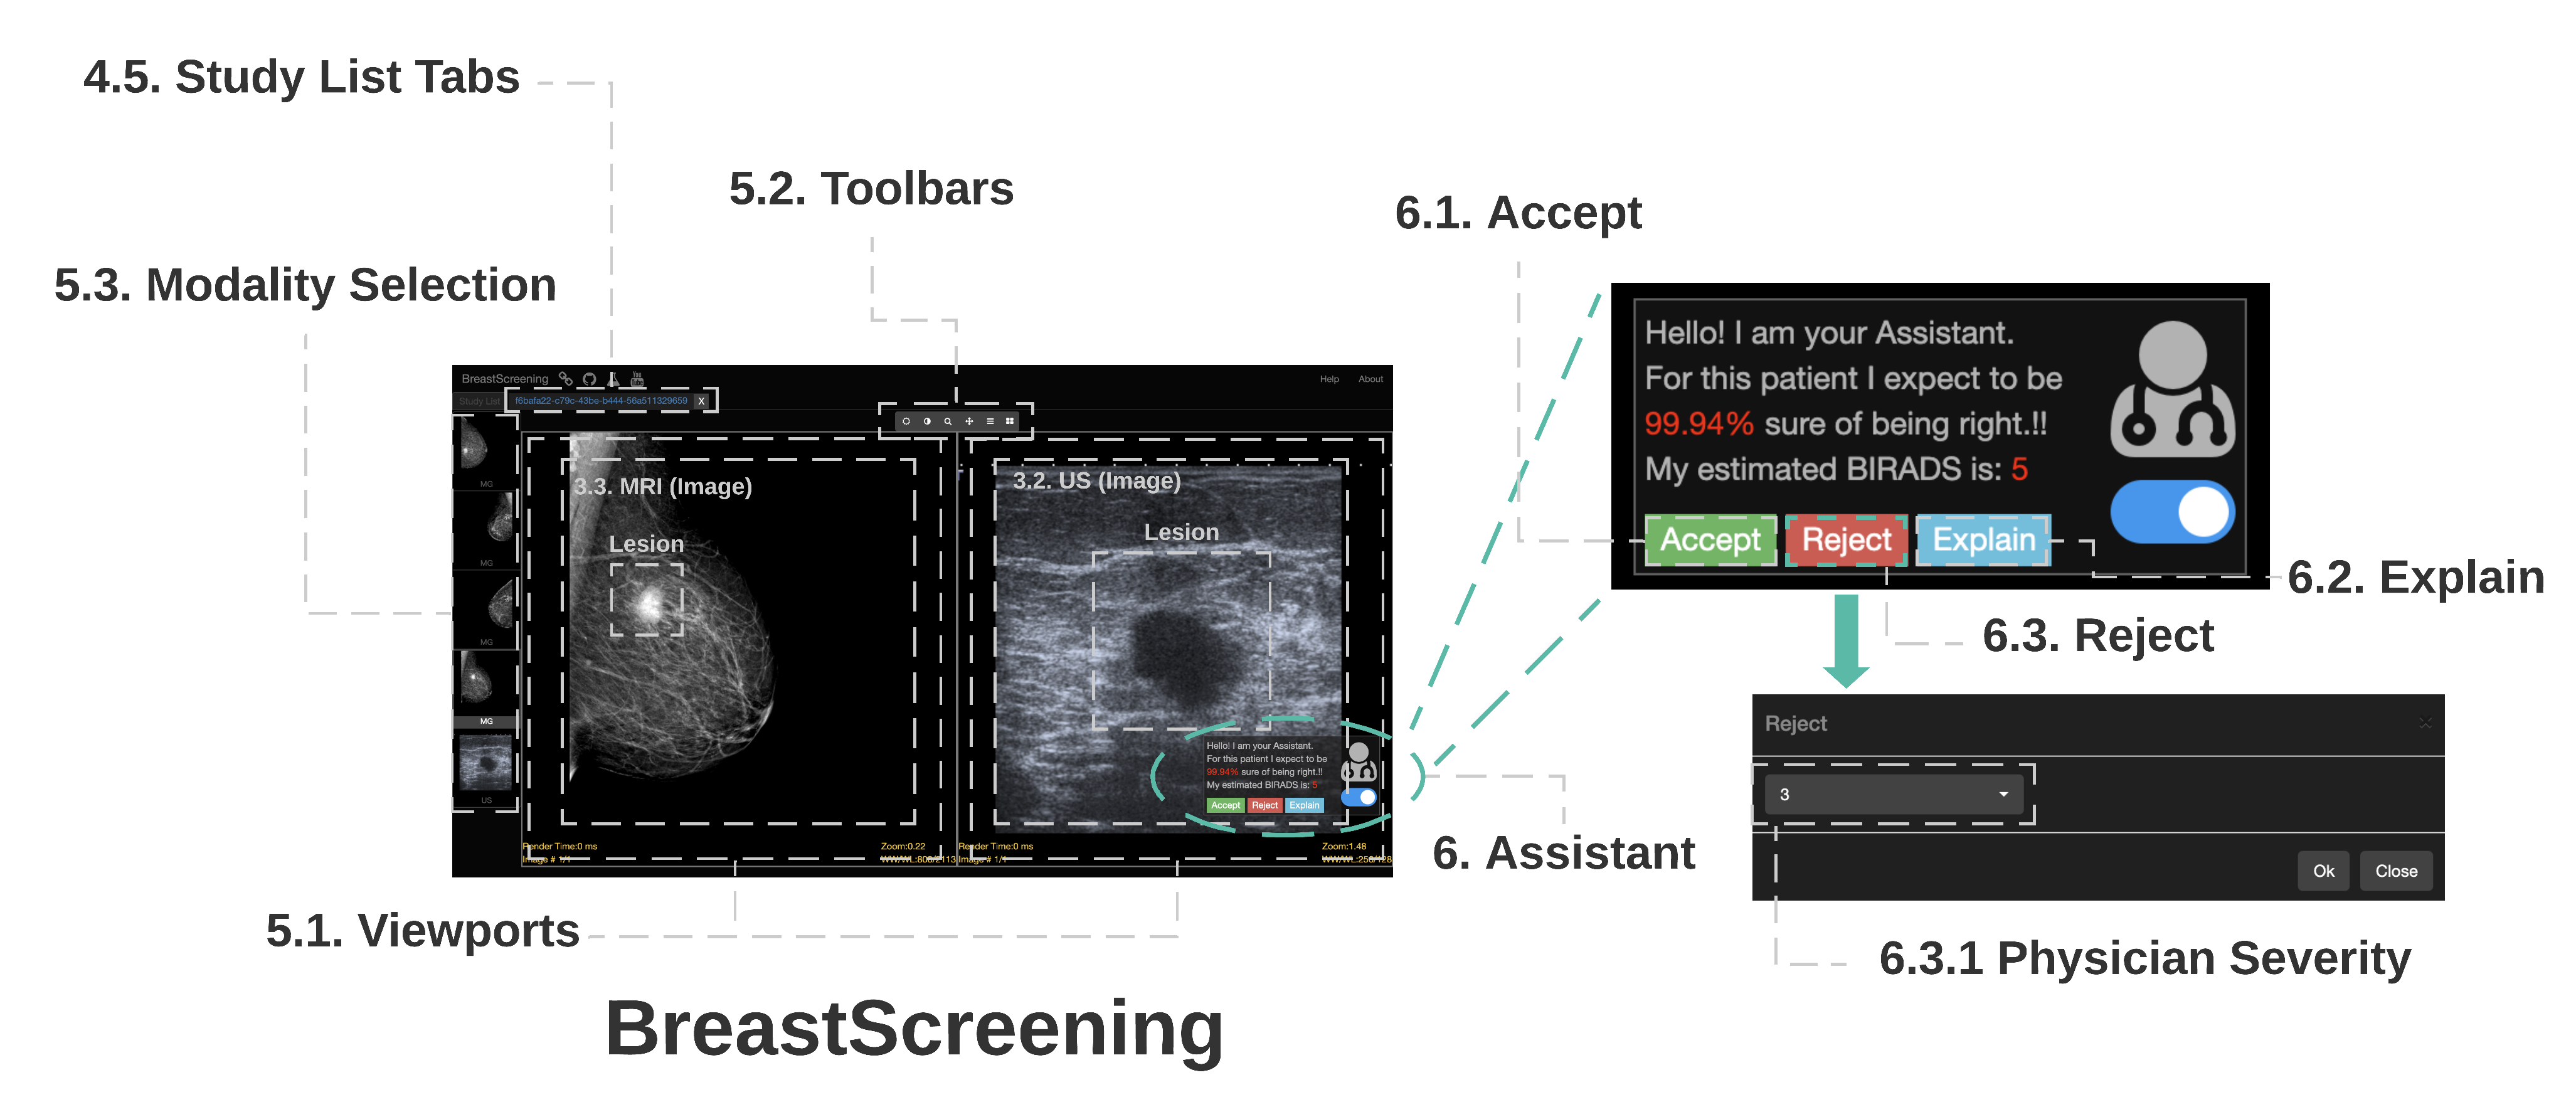
\includegraphics[width=0.95\textwidth]{fig002}
\caption{Our {\it BreastScreening} assistant provides several features regarding the basics of {\it Radiomics}. From there, we will be able to validate our DenseNet BIRADS classifier along with clinicians.}
\label{fig:fig002}
\twocolumn
\end{figure}
%%%%%%%%%%%%%%%%%%%%%%%%%%%%%%%%%%%%%%%%%%%%%%%%%%%